\documentclass[a4paper, 11pt]{article}
%\usepackage{qtree} %z jakiegoś dziwacznego powodu ten pakiet musi być aż tak wysoko...
\usepackage[OT4,plmath,MeX]{polski}
\usepackage{amstext, amsopn, amsfonts, amsthm, amsbsy, latexsym, amssymb}
\usepackage[utf8]{inputenc}

\usepackage{indentfirst}
\usepackage[margin=2cm]{geometry}
\usepackage{amsmath} %found in http://en.wikibooks.org/wiki/LaTeX/Formatting
\usepackage{amsfonts}
\usepackage{amssymb}
\usepackage{enumerate}
\usepackage{textcomp}

\usepackage{multirow}

\usepackage{graphicx}
\usepackage{epstopdf}
\usepackage{url}
\usepackage{hyperref}
\usepackage{multirow}
\usepackage{listings}

\begin{document}

\title{Raport z projektu Analizatora EKG}
\author{Mateusz Baran \and
Krzysztof Bębenek \and
Bartłomiej Bułat \and
Szczepan Czaicki \and
Tomasz Drzewiecki \and
Krzysztof Farganus \and
Łukasz Jaromi \and
Mateusz Krasucki \and
Łukasz Krzyżek \and
Łukasz Kutrzuba \and
Weronika Łabaj \and
Paweł Maślanka \and
Piotr Matuszkiewicz \and
Norbert Pabian \and
Łukasz Pękala \and
Krzysztof Piekutowski \and
Grzegorz Pietrzyk \and
Łukasz Podolski \and
Mikołaj Rzepka \and
Agata Sitnik \and
Leszek Sosnowski \and
Aleksander Steliga \and
Mateusz Ślażyński \and
Łukasz Zieńkowski}


\maketitle
\newpage

\tableofcontents
\newpage

\section{Specyfikacja zadania}

Celem projektu jest stworzenie zintegrowanego systemu pozwalającego na przeglądanie i automatyczną analizę sygnału EKG. Sygnał dostarczany jest w formie cyfrowej w standardzie wykorzystywanym w MIT–BIH Arrhythmia Database. Różne etapy przetwarzania, takie jak usuwanie linii bazowej, detekcja załamków R czy klasyfikacja zespołów QRS wykonywana jest przez różne zespoły (szczegółowe opisy specyfikacji modułów: \ref{sec:mod}), których praca składa się na jeden program.

Moduły przetwarzania integrowane i uzupełniane są modułami kontrolującymi przepływ danych i odpowiadającymi za komunikację z użytkownikiem. Wzajemne zależności pomiędzy modułami prezentuje rys. \ref{fig:zaleznosci}.

\begin{figure}[h!]
  \centering
  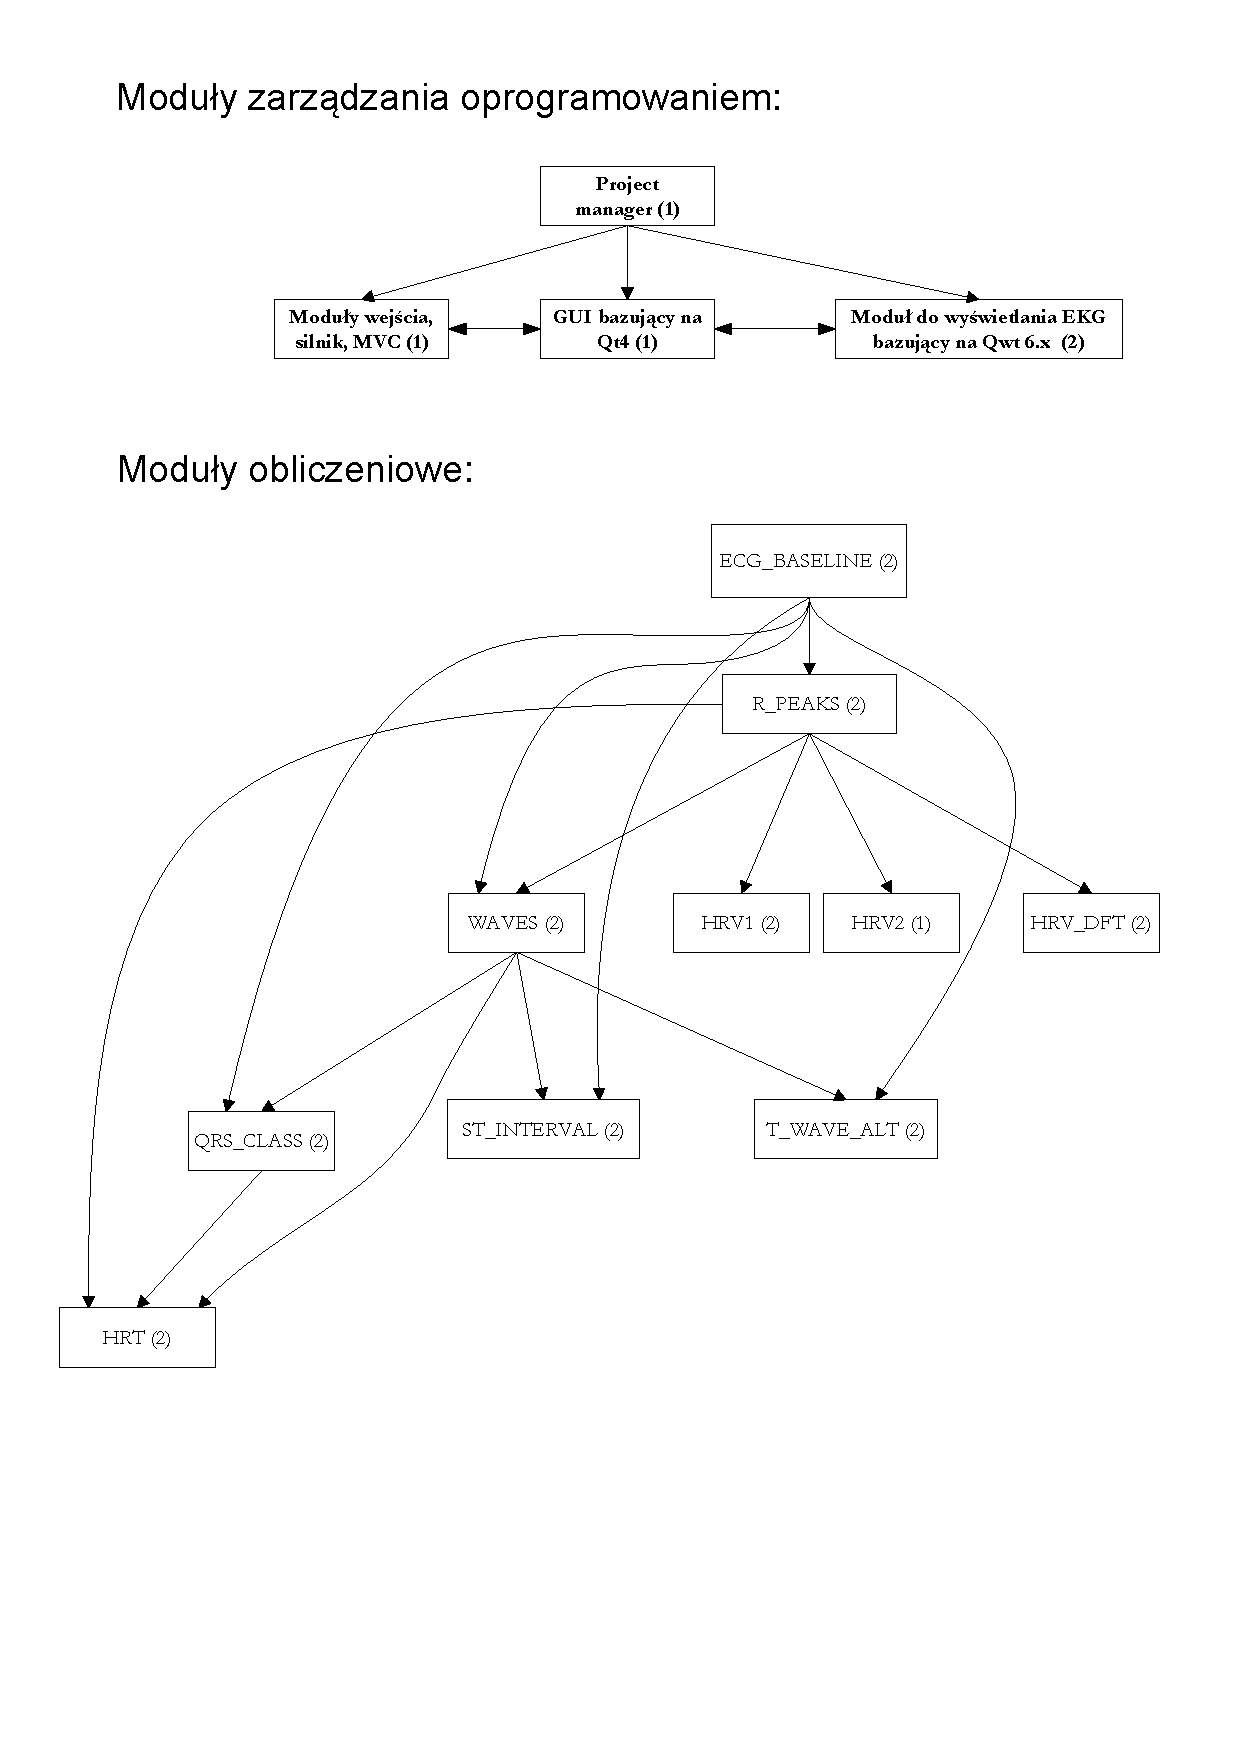
\includegraphics[width=0.7\linewidth]{include/Projekt_zaleznosci}
  \label{fig:zaleznosci}
  \caption{Zależności pomiędzy modułami projektu.}
\end{figure}

\section{Specyfikacja techniczna rozwiązania}
\label{sec:techspec}

\subsection{Wykorzystane narzędzia}
\label{sec:tools}

Podczas realizacji projektu wykorzystywane były różne narzędzia do tworzenia i prototypowania rozwiązań. Wstępne projekty przygotowywane były w programie Matlab, zaś ostateczny kod powstawał w języku C++ (standard '03 z elementami standardu C++11 obsługiwanymi przez wspierane kompilatory).
Minimalne wymagania kompilacji projektu są następujące:
\begin{itemize}
  \item Jeden z kompilatorów:
  \begin{itemize}
    \item Microsoft Visual Studio 2010
    \item GCC 4.5
  \end{itemize}
  \item Biblioteki:
  \begin{itemize}
    \item Boost 1.51
    \item Qt 4.8
    \item Qwt 6.01
    \item gsl 1.15
    \item WFDB 10.5.16 (zawarta w źródłach projektu)
    \item FFTW 3.3.2
  \end{itemize}
\end{itemize}

Do wersjonowania i śledzenia błędów wykorzystywaliśmy platformę Github wraz z rozproszonym systemem kontroli wersji Git. Posiada on zaawansowane możliwości wspierające pracę grupową nad projektem, co szczególnie przydaje się, gdy liczba osób jest duża.

\subsection{Projekt systemu}
\label{sec:sys_proj}

Program został wykonany w architekturze MVC -- istnieje ścisły podział na część wyświetlającą interfejs użytkownika, moduły przetwarzania sygnału oraz kontroler łączący te dwa elementy, co obrazuje diagram pakietów \ref{fig:package_diagram}. Zastosowano obiektowe podejście przy projektowaniu hierarchii klas realizujących przetwarzanie (rys. \ref{fig:class_diagram}), umożliwiające bezproblemową wymianę implementacji dowolnego modułu na inną.

\begin{figure}[h!]
  \centering
  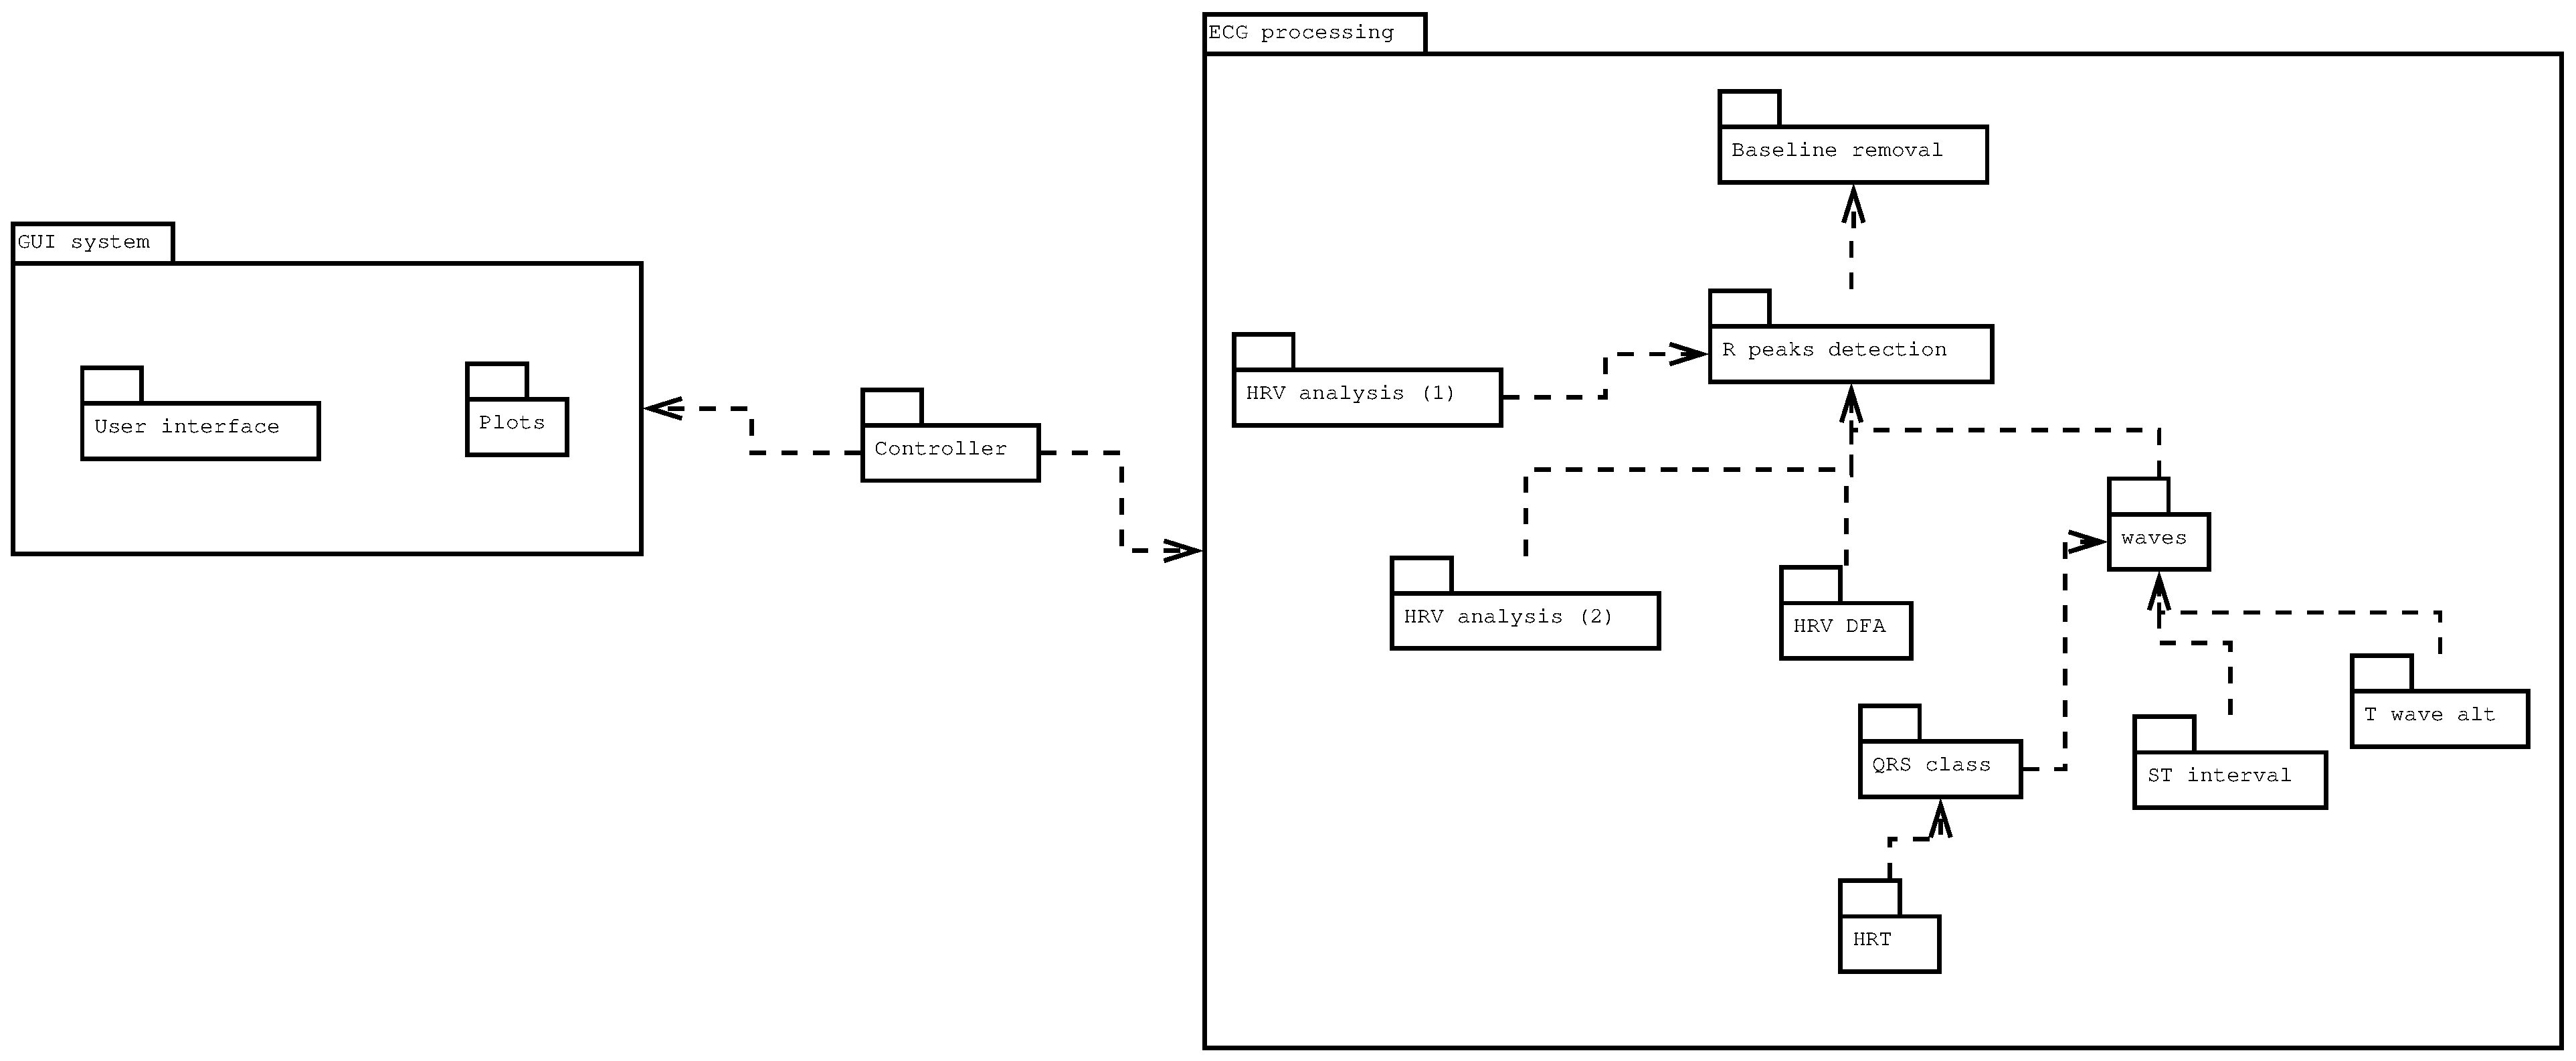
\includegraphics[width=\linewidth]{include/package_diagram}
  \label{fig:package_diagram}
  \caption{Diagram pakietów.}
\end{figure}

Samo przetwarzanie realizowane jest wielofazowo -- moduły przeliczane są sekwencyjnie na osobnym wątku niż wątek zdarzeń GUI, co pozwala na zatrzymanie zbyt długo trwającej operacji. Zaimplementowano także mechanizm buforowania wyników, dzięki czemu przy zmianie parametrów pewnego modułu nie ma konieczności przeliczania wyników modułów wcześniejszych.

Cała aplikacja napisana jest jako samodzielny, wieloplatformowy program (rys. \ref{fig:deployment_diagram}) -- możliwa jest kompilacja pliku binarnego pod systemami Windows, Linux i MacOS X. Całe przetwarzanie wykonywane jest lokalnie, dzięki czemu nie jest wymagane połączenie z Internetem. Dzięki wybraniu licencji GPL v2+ projekt jest wolny i możliwy jest jego dalszy rozwój i kompilacja na nowe platformy.

\begin{figure}[h!]
  \centering
  \includegraphics[width=0.5\linewidth]{include/deployment_diagram}
  \label{fig:deployment_diagram}
  \caption{Diagram wdrożenia.}
\end{figure}

\section{Opisy modułów}
\label{sec:mod}

\subsection{Usuwanie linii bazowej}
\label{sec:baseline}
Autorzy: Weronika Łabaj i Piotr Matuszkiewicz.

\subsubsection{Opis zadania}
\label{sec:baseline:desc}

\begin{description}
\item[Temat] Metody filtracji i detekcji izolinii w sygnale EKG
\item[Opis] Występujące zakłócenia sieciowe i mięśniowe, jak również falowanie linii izoelektrycznej w sygnale EKG niejednokrotnie uniemożliwiają właściwą i poprawną analizę sygnału. Celem projektu jest opracowanie i implementacja metod związanych filtracją i detekcją linii izoelektrycznej w sygnale EKG. W szczególności należy rozważyć:
  \begin{itemize}
  \item filtr Butterwortha,
  \item średnią kroczącą,
  \item metody nieadaptacyjne: filtr Savitzky-Golay’a
  \item metody atapdacyjne np. filtr Wienera, LMS
  \end{itemize}
\item[Dane] ciąg próbek sygnału EKG z bazy Physionet.org
\item[Szukane] moduł programu filtrujący sygnał EKG z zakłóceń sieciowych/mięśniowych oraz usuwający z sygnału falowanie linii izoelektrycznej przy wykorzystaniu różnych metod; w ostatecznym module programu będzie możliwość wyboru algorytmu filtrującego i usuwającego falowanie linii izoelektrycznej
\end{description}

\subsubsection{Badania literaturowe}
\label{sec:baseline:papers}

\subsubsection{Opis procedur i metod}
\label{sec:baseline:procs}

\subsubsection{Warunki testowania}
\label{sec:baseline:tests}

\subsubsection{Wyniki}
\label{sec:baseline:results}

\subsection{Wykrywanie załamków R}
\label{sec:Rs}

\subsection{Waves}
\label{sec:waves}

\subsection{HRV1}
\label{sec:hrv1}

\subsection{HRV2}
\label{sec:hrv2}

\subsection{HRV DFA}
\label{sec:hrvd_fa}

\subsection{Klasyfikacja zespołów QRS}
\label{sec:qrs_class}

\subsection{ST interval}
\label{sec:st_interval}

\subsection{T wave alt}
\label{sec:t_wave_alt}

\subsection{HRT}
\label{sec:hrt}

\end{document}